\documentclass[spanish]{article}
\usepackage{amsmath, amsfonts, amsthm}
\usepackage{float}
\usepackage{tikz}
\usepackage{hyperref}
\usetikzlibrary{automata, arrows, arrows.meta, positioning, babel, shapes.misc}
\tikzset{shorten >= 1pt,
         node distance = 3cm, on grid,
         >= stealth,
         every initial
           by arrow/.style = -{Straight Barb[length = 1.1ex]},
         initial text = {},
         initial distance = 0.05,
         every state/.style = {minimum size = 5mm},
         bend angle = 20,
         every loop/.style = {looseness = 13}}

\newcommand{\tnum}{2}
\begin{document}

\title{
    Tarea 4 \\
    Informática Teórica
}
\author{
    Matías Peñaloza
    202373037-8
}
\date{
    2024-2
}
\maketitle

\begin{center}
  \begin{tabular}{|l|r|}
    \hline
    \multicolumn{1}{|c|}{\textbf{Concepto}} &
      \multicolumn{1}{c|}{\textbf{Tiempo [min]}} \\
    \hline
    Revisión & 60\\
    \hline
    Desarrollo    & 90\\
    \hline
    Informe	      & 90\\
    \hline
  \end{tabular}
\end{center}

\section{Enunciado}
Directamente construya autómatas de pila
  que acepten los siguientes lenguajes,
  ya sea por estado final o por pila vacía.
  Explique sus construcciones.
  \begin{enumerate}
  \item % 20242t4p1
    \(L_1 = \{a^i b^j c^k \colon i + j = k\}\)
    \\ \hspace*{\fill}(50 puntos)
  \item % 20242t4p2
    \(L_2 = \{\omega \in \{a, b\}^* \colon \#_a((\omega) \ne \#_b(\omega)\}\),
    donde \(\#_a(\omega)\) es el número de \(a\) en \(\omega\).
    \\ \textbf{Pista:}
    Contabilice la diferencia del número de \(a\) y \(b\) vistas,
    por ejemplo con \(A\) en la pila las \(a\) sobrantes
    y con \(B\) las \(b\) sobrantes.
    \\ \hspace*{\fill}(50 puntos)
  \item % 20242t4p3
    ¿Son deterministas sus autómatas?
    \\ \hspace*{\fill}(20 puntos)
  \end{enumerate}

\section{Desarrollo}
\subsection{PDA $M_1$ para $L_1$}
  Para la estructura partiremos de la idea de aceptar los caracteres en el orden $a$, $b$, $c$ y
  aceptar que $i$, $j$ o $k$ podrian ser $0$ en algunos casos. Resultando en el siguiente automata:
  \begin{figure}[H]
    \centering
    \label{fig:figura1}
    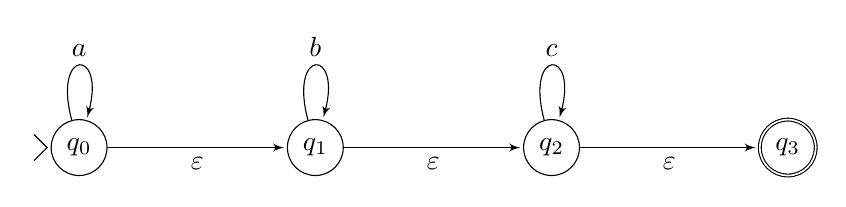
\begin{tikzpicture}
        \node[state, initial]   (q0)                    {$q_0$};
        \node[state]            (q1) [right of = q0]    {$q_1$};
        \node[state]            (q2) [right of = q1]    {$q_2$};
        \node[state, accepting] (q3) [right of = q2]    {$q_3$};
        
        \path[-latex']          (q0) edge[loop above]   node[above] {$a$}  (q0);
        \path[-latex']          (q1) edge[loop above]   node[above] {$b$}  (q1);
        \path[-latex']          (q2) edge[loop above]   node[above] {$c$}  (q2);

        \path[-latex']          (q0) edge               node[below] {$\varepsilon$} (q1);
        \path[-latex']          (q1) edge               node[below] {$\varepsilon$} (q2);
        \path[-latex']          (q2) edge               node[below] {$\varepsilon$} (q3);
    \end{tikzpicture}
    \caption{Automata orden $a$, $b$, $c$}
  \end{figure}
  Para la pila (con el simbolo inicial $\mathbb{Z}_0$) podemos insertar una $X$ cada vez que veamos una $a$ o una $b$ y
  luego quitar las $X$ cada vez que vemos una $c$, lo que nos llevara a tener $\mathbb{Z}_0$ para el estado final de aceptacion
  solamente si la cantidad de $a's$ mas las de $b's$ son igual a la cantidad de $c's$.\\
  Por lo tanto transformamos las transiciones con $a$ a las siguientes:
  \begin{itemize}
    \item $a, X / XX$
    \item $a, \mathbb{Z}_0 / \mathbb{Z}_0 X$
  \end{itemize}
  las transiciones con $b$ a:
  \begin{itemize}
    \item $b, X / XX$
    \item $b, \mathbb{Z}_0 / \mathbb{Z}_0 X$
  \end{itemize}
  las transiciones con $c$ a:
  \begin{itemize}
    \item $c, X / \varepsilon$
  \end{itemize}
  y por ultimo las transiciones con $\varepsilon$ no deben afectar la pila:
  \begin{itemize}
    \item $\varepsilon, X / X$
    \item $\varepsilon, \mathbb{Z}_0 / \mathbb{Z}_0$
  \end{itemize}
  Resultando en el siguiente automata de pila $M_1$:
  \begin{figure}[H]
    \centering
    \label{fig:figura2}
    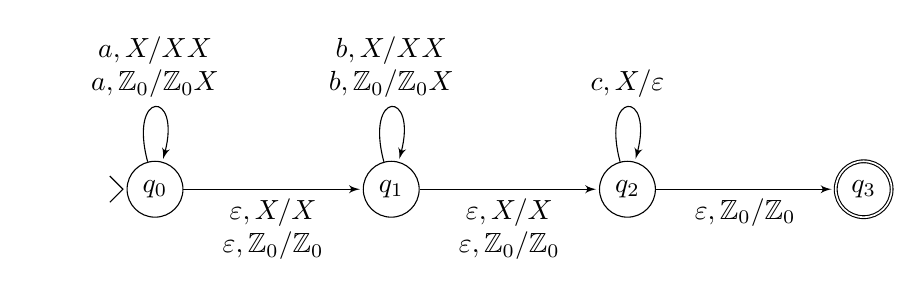
\begin{tikzpicture}
        \node[state, initial]   (q0)                    {$q_0$};
        \node[state]            (q1) [right of = q0]    {$q_1$};
        \node[state]            (q2) [right of = q1]    {$q_2$};
        \node[state, accepting] (q3) [right of = q2]    {$q_3$};
        
        \path[-latex']          (q0) edge[loop above]   node[above] {\parbox{3cm}{\centering $a, X / XX$ \\ $a, \mathbb{Z}_0 / \mathbb{Z}_0 X$}}  (q0);
        \path[-latex']          (q1) edge[loop above]   node[above] {\parbox{3cm}{\centering $b, X / XX$ \\ $b, \mathbb{Z}_0 / \mathbb{Z}_0 X$}}  (q1);
        \path[-latex']          (q2) edge[loop above]   node[above] {$c, X / \varepsilon$}  (q2);

        \path[-latex']          (q0) edge               node[below] {\parbox{3cm}{\centering $\varepsilon, X / X$ \\ $\varepsilon, \mathbb{Z}_0 / \mathbb{Z}_0$}} (q1);
        \path[-latex']          (q1) edge               node[below] {\parbox{3cm}{\centering $\varepsilon, X / X$ \\ $\varepsilon, \mathbb{Z}_0 / \mathbb{Z}_0$}} (q2);
        \path[-latex']          (q2) edge               node[below] {$\varepsilon, \mathbb{Z}_0 / \mathbb{Z}_0$} (q3);
    \end{tikzpicture}
    \caption{PDA $M_1$}
  \end{figure}

\subsection{PDA $M_2$ para $L_2$}
  Para la estructura partiremos del automata que acepta $L(a^*b^*)$ con una transicion $\varepsilon$:
  \begin{figure}[H]
    \centering
    \label{fig:figura3}
    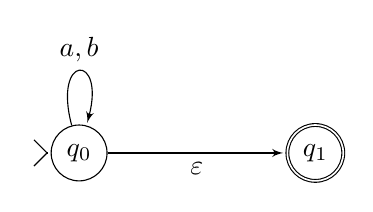
\begin{tikzpicture}
        \node[state, initial]   (q0)                          {$q_0$};
        \node[state, accepting] (q1) [right of = q0]          {$q_1$};

        \path[-latex']          (q0) edge[loop above]   node[above] {$a, b$} (q0);
        \path[-latex']          (q0) edge               node[below] {$\varepsilon$} (q1);
    \end{tikzpicture}
    \caption{Automata $a^*b^*$}
  \end{figure}
  Para la pila utilizaremos la pista y agregaremos $A's$ para las $a's$ sobrantes y $B's$
  para las $b's$ sobrantes, ademas deberemos de quitar una $A$ si encontramos una $b$ (que compensa a la $a$ sobrante) y viceversa.
  Asi entonces transformamos las transiciones con $a$ a las siguientes:
  \begin{itemize}
    \item $a, \mathbb{Z}_0 / \mathbb{Z}_0 A$
    \item $a, A / AA$
    \item $a, B / \varepsilon$
  \end{itemize}
  las transiciones con $b$ a:
  \begin{itemize}
    \item $b, \mathbb{Z}_0 / \mathbb{Z}_0 B$
    \item $b, B / BB$
    \item $b, A / \varepsilon$
  \end{itemize}
  y las transiciones con $\varepsilon$ tendran que llevarnos al estado
  de aceptacion unicamente si existe una $A$ o una $B$ ($a$ o $b$ sobrante)
  al tope de la pila, de esta manera no se aceptaran cantidades iguales de $a's$ y $b's$:
  \begin{itemize}
    \item $\varepsilon, A / A$
    \item $\varepsilon, B/ B$
  \end{itemize}
  Finalmente nuestro PDA $M_2$ resultante:
  \begin{figure}[H]
    \centering
    \label{fig:figura4}
    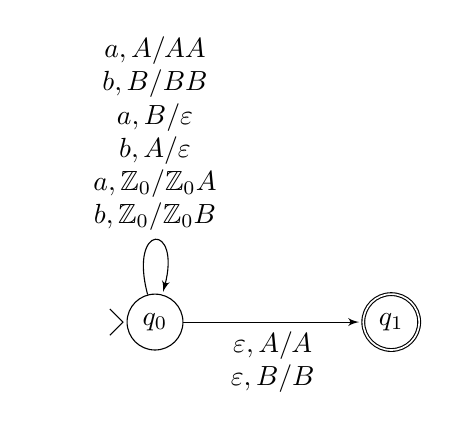
\begin{tikzpicture}
        \node[state, initial]   (q0)                          {$q_0$};
        \node[state, accepting] (q1) [right of = q0]          {$q_1$};

        \path[-latex']          (q0) edge[loop above]   node[above] {\parbox{3cm}{\centering $a, A / AA$\\$b, B / BB$\\$a, B / \varepsilon$\\$b, A / \varepsilon$\\$a, \mathbb{Z}_0 / \mathbb{Z}_0 A$\\$b, \mathbb{Z}_0 / \mathbb{Z}_0 B$}} (q0);
        \path[-latex']          (q0) edge               node[below] {\parbox{3cm}{\centering $\varepsilon, A / A$ \\ $\varepsilon, B / B$}} (q1);
    \end{tikzpicture}
    \caption{PDA $M_2$}
  \end{figure}

\subsection{¿PDA's $M_1$ y $M_2$ deterministas?}
  Para saber si los PDA's son deterministas basta con fijarse en sus estructuras con las cuales los armamos.
  Para el PDA $M_1$ podemos ver que el automata con el cual lo construimos (ver Figura~\ref{fig:figura1}) es un NFA ya
  que el automata tiene que decidir entre leer un caracter o leer $\varepsilon$, esto mismo se aplica para la estructura
  con la cual armamos al PDA $M_2$ (ver Figura~\ref{fig:figura3}).
  Por lo tanto ninguno de nuestros PDA's son deterministas.

\end{document}